\documentclass[tikz,border=4pt]{standalone}
\usepackage{ctex}
\usepackage{amsmath}
\usetikzlibrary{calc, arrows.meta, angles, quotes}

\begin{document}
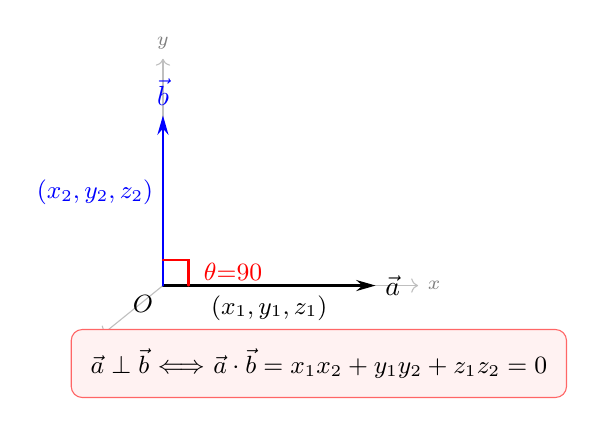
\begin{tikzpicture}[
  x={(1.8cm,0cm)},
  y={(0cm,1.8cm)},
  z={(-0.52cm,-0.42cm)},
  line cap=round,
  vec/.style={-{Stealth[length=7pt, width=4pt]}, thick},
  vecblue/.style={-{Stealth[length=7pt, width=4pt]}, thick, blue},
]

% 空间向量垂直判定示意图
% 共起点 O，向量 a 和 b 夹角 θ = 90°

\coordinate (O) at (0,0,0);

% 向量 a：沿接近 x 轴偏一点（等距投影中显示立体感）
\coordinate (Aend) at (1.5,0,0);

% 向量 b：垂直于 a（在 y-z 平面内）
\coordinate (Bend) at (0,1.2,0);

% 坐标系轴（淡灰色参考）
\draw[gray!50, thin, ->] (0,0,0) -- (1.8,0,0) node[right, font=\scriptsize, gray] {$x$};
\draw[gray!50, thin, ->] (0,0,0) -- (0,1.6,0) node[above, font=\scriptsize, gray] {$y$};
\draw[gray!50, thin, ->] (0,0,0) -- (0,0,1.5) node[below left, font=\scriptsize, gray] {$z$};

% 画向量 a
\draw[vec, black] (O) -- (Aend);
\node[right, font=\normalsize] at (Aend) {$\vec{a}$};

% 画向量 b
\draw[vecblue] (O) -- (Bend);
\node[above, font=\normalsize, blue] at (Bend) {$\vec{b}$};

% 直角标记（θ = 90°）
\coordinate (rpt1) at (0.18,0,0);
\coordinate (rpt2) at (0.18,0.18,0);
\coordinate (rpt3) at (0,0.18,0);
\draw[red, thick] (rpt1) -- (rpt2) -- (rpt3);

% θ = 90° 标注
\node[right, font=\small, red] at (0.22, 0.10, 0) {$\theta{=}90°$};

% 原点标注
\node[below left, font=\small] at (O) {$O$};

% 分量标注（a 和 b 的坐标）
\node[below, font=\small, black] at ($(O)!0.5!(Aend)$) {$(x_1,y_1,z_1)$};
\node[left, font=\small, blue] at ($(O)!0.55!(Bend)$) {$(x_2,y_2,z_2)$};

% 公式框
\node[draw=red!60, fill=red!5, rounded corners=4pt,
      align=center, font=\small, inner sep=7pt] at (1.1,-0.55,0)
  {$\vec{a}\perp\vec{b}$ $\Longleftrightarrow$
   $\vec{a}\cdot\vec{b}=x_1x_2+y_1y_2+z_1z_2=0$};

\end{tikzpicture}
\end{document}
